\chapter{Setup BaseCam Controller}

\addthumb{\LARGE\quad Setup BaseCam Controller}{\Huge \textbf{  \ding{223}}}{white}{titlepagecolor!25}

\section{Our setup}
Using the system with a mounted Lumix FZ200 and manual tuning, we reached an optimal configuration for the tunable values of the BaseCam SimpleBGC. Depending on motors, camera weight and camera positioning, these may vary a lot. It is recommended to follow the procedures as described in the following section as well as any procedures specific to your electronics.

\section{Basic}
In the first tab, the first thing to enter are the motor configuration parameters. The POWER should be set according to the motors capabilities. The value ranges from 1-255, where 255 equals the full voltage from the battery. The + value may be set to allow the controller to momentarily provide the motor with additional voltage, though the sum of POWER and + may maximally be 255.\par
The NUM. POLES needs to be set to the number of poles of the used motors. For our motors, this value is 22.\par
For the sensor, the alignment of the IMU needs to be considered. If assembly was completed according to instructions, Axis TOP should be –Z and RIGHT should be –Y. For other setups of IMU models, consult the orientation of the IMU.\par
The PID controller requires extensive manual calibration. It is recommended to tune the axes sequentially. Start with tuning the ROLL axis and set the power of PITCH and YAW to 1. Initials values can be set to P=10, I=0.01, D=10. Begin manual tuning and follow recommended guidelines. Increase the values, first P, then D, then I to obtain their maximally stable values. To observe the effect, go to the Realtime Data tab and observe the oscillations. For further instructions on manual tuning, we refer to the SimpleBGC Manual. \footnote{\url{http://www.basecamelectronics.com/downloads/}}
For reference, see the screenshot \ref{SRNSHOT:BGCMain} with the settings used on our \textbf{\textsf{OpenSAM}}.
\begin{figure}[!h]
    \centering
    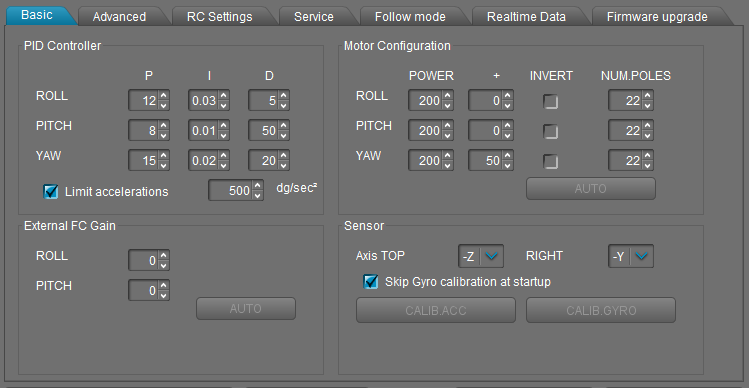
\includegraphics[width=0.8\textwidth]{BGCSetup/SimpleBGCMain.PNG}
    \label{SRNSHOT:BGCMain}
    \caption{Screenshot of SimpleBGC Basic tab}
\end{figure}

\section{Advanced}
In the Advanced tab, under Motor Outputs, the YAW should be set to YAW ext. board. Under timings, the PWM frequency needs to be set to HIGH (silent).

\section{RC Settings}
In RC Settings, map the joystick analog PITCH and ROLL inputs to the PITCH and YAW of the gimbal. Limit the RCCONTROL values to the maximally stable values of your system. The button on the Joystick was mapped to begin calibration of the gyroscope, accelerometer and to turn motors on/off. See screenshots \ref{SRNSHOT:BGCjoystick}.

\begin{figure*}[!h]
    \centering
    \begin{subfigure}
        \raggedleft
        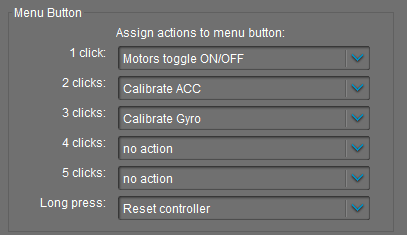
\includegraphics[width=0.4\textwidth]{BGCSetup/SimpleBGCMenu.PNG}
    \end{subfigure}%
    \begin{subfigure}
        \raggedright
        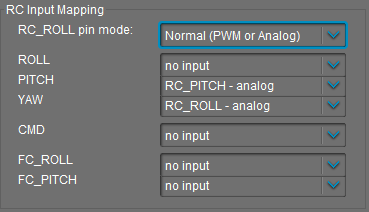
\includegraphics[width=0.4\textwidth]{BGCSetup/SimpleBGCRCInput.PNG}
    \end{subfigure}
\end{figure*}
\vspace{-0.5cm}
\begin{figure}[!h]
    \centering
    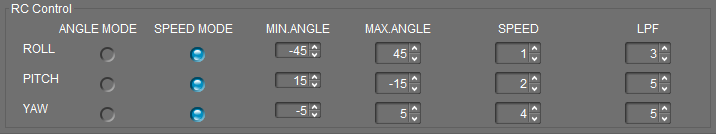
\includegraphics[width=0.8\textwidth]{BGCSetup/SimpleBGCRCControl.PNG}
    \label{SRNSHOT:BGCjoystick}
    \caption{Screenshot of SimpleBGC Basic tab}
\end{figure}

\section{Service}
In the Service tab, specify the joystick’s menu button commands and set your battery monitoring values according to your battery’s specifications.

